
\documentclass[12pt,journal,compsoc,onecolumn]{thesis}

% *** MISC UTILITY PACKAGES ***
%
%\usepackage{ifpdf}
% Heiko Oberdiek's ifpdf.sty is very useful if you need conditional
% compilation based on whether the output is pdf or dvi.
% usage:
% \ifpdf
%   % pdf code
% \else
%   % dvi code
% \fi
% The latest version of ifpdf.sty can be obtained from:
% http://www.ctan.org/pkg/ifpdf
% Also, note that IEEEtran.cls V1.7 and later provides a builtin
% \ifCLASSINFOpdf conditional that works the same way.
% When switching from latex to pdflatex and vice-versa, the compiler may
% have to be run twice to clear warning/error messages.

% *** CITATION PACKAGES ***
%
\ifCLASSOPTIONcompsoc
  % IEEE Computer Society needs nocompress option
  % requires cite.sty v4.0 or later (November 2003)
  \usepackage[nocompress]{cite}
\else
  % normal IEEE
  \usepackage{cite}
\fi
% cite.sty was written by Donald Arseneau
% V1.6 and later of IEEEtran pre-defines the format of the cite.sty package
% \cite{} output to follow that of the IEEE. Loading the cite package will
% result in citation numbers being automatically sorted and properly
% "compressed/ranged". e.g., [1], [9], [2], [7], [5], [6] without using
% cite.sty will become [1], [2], [5]--[7], [9] using cite.sty. cite.sty's
% \cite will automatically add leading space, if needed. Use cite.sty's
% noadjust option (cite.sty V3.8 and later) if you want to turn this off
% such as if a citation ever needs to be enclosed in parenthesis.
% cite.sty is already installed on most LaTeX systems. Be sure and use
% version 5.0 (2009-03-20) and later if using hyperref.sty.
% The latest version can be obtained at:
% http://www.ctan.org/pkg/cite
% The documentation is contained in the cite.sty file itself.
%
% Note that some packages require special options to format as the Computer
% Society requires. In particular, Computer Society  papers do not use
% compressed citation ranges as is done in typical IEEE papers
% (e.g., [1]-[4]). Instead, they list every citation separately in order
% (e.g., [1], [2], [3], [4]). To get the latter we need to load the cite
% package with the nocompress option which is supported by cite.sty v4.0
% and later. Note also the use of a CLASSOPTION conditional provided by
% IEEEtran.cls V1.7 and later.





% *** GRAPHICS RELATED PACKAGES ***
%
\ifCLASSINFOpdf
  % \usepackage[pdftex]{graphicx}
  % declare the path(s) where your graphic files are
  % \graphicspath{{../pdf/}{../jpeg/}}
  % and their extensions so you won't have to specify these with
  % every instance of \includegraphics
  % \DeclareGraphicsExtensions{.pdf,.jpeg,.png}
\else
  % or other class option (dvipsone, dvipdf, if not using dvips). graphicx
  % will default to the driver specified in the system graphics.cfg if no
  % driver is specified.
  % \usepackage[dvips]{graphicx}
  % declare the path(s) where your graphic files are
  % \graphicspath{{../eps/}}
  % and their extensions so you won't have to specify these with
  % every instance of \includegraphics
  % \DeclareGraphicsExtensions{.eps}
\fi
% graphicx was written by David Carlisle and Sebastian Rahtz. It is
% required if you want graphics, photos, etc. graphicx.sty is already
% installed on most LaTeX systems. The latest version and documentation
% can be obtained at: 
% http://www.ctan.org/pkg/graphicx
% Another good source of documentation is "Using Imported Graphics in
% LaTeX2e" by Keith Reckdahl which can be found at:
% http://www.ctan.org/pkg/epslatex
%
% latex, and pdflatex in dvi mode, support graphics in encapsulated
% postscript (.eps) format. pdflatex in pdf mode supports graphics
% in .pdf, .jpeg, .png and .mps (metapost) formats. Users should ensure
% that all non-photo figures use a vector format (.eps, .pdf, .mps) and
% not a bitmapped formats (.jpeg, .png). The IEEE frowns on bitmapped formats
% which can result in "jaggedy"/blurry rendering of lines and letters as
% well as large increases in file sizes.
%
% You can find documentation about the pdfTeX application at:
% http://www.tug.org/applications/pdftex






% *** MATH PACKAGES ***
%
%\usepackage{amsmath}
% A popular package from the American Mathematical Society that provides
% many useful and powerful commands for dealing with mathematics.
%
% Note that the amsmath package sets \interdisplaylinepenalty to 10000
% thus preventing page breaks from occurring within multiline equations. Use:
%\interdisplaylinepenalty=2500
% after loading amsmath to restore such page breaks as IEEEtran.cls normally
% does. amsmath.sty is already installed on most LaTeX systems. The latest
% version and documentation can be obtained at:
% http://www.ctan.org/pkg/amsmath





% *** SPECIALIZED LIST PACKAGES ***
%
%\usepackage{algorithmic}
% algorithmic.sty was written by Peter Williams and Rogerio Brito.
% This package provides an algorithmic environment fo describing algorithms.
% You can use the algorithmic environment in-text or within a figure
% environment to provide for a floating algorithm. Do NOT use the algorithm
% floating environment provided by algorithm.sty (by the same authors) or
% algorithm2e.sty (by Christophe Fiorio) as the IEEE does not use dedicated
% algorithm float types and packages that provide these will not provide
% correct IEEE style captions. The latest version and documentation of
% algorithmic.sty can be obtained at:
% http://www.ctan.org/pkg/algorithms
% Also of interest may be the (relatively newer and more customizable)
% algorithmicx.sty package by Szasz Janos:
% http://www.ctan.org/pkg/algorithmicx




% *** ALIGNMENT PACKAGES ***
%
%\usepackage{array}
% Frank Mittelbach's and David Carlisle's array.sty patches and improves
% the standard LaTeX2e array and tabular environments to provide better
% appearance and additional user controls. As the default LaTeX2e table
% generation code is lacking to the point of almost being broken with
% respect to the quality of the end results, all users are strongly
% advised to use an enhanced (at the very least that provided by array.sty)
% set of table tools. array.sty is already installed on most systems. The
% latest version and documentation can be obtained at:
% http://www.ctan.org/pkg/array


% IEEEtran contains the IEEEeqnarray family of commands that can be used to
% generate multiline equations as well as matrices, tables, etc., of high
% quality.




% *** SUBFIGURE PACKAGES ***
%\ifCLASSOPTIONcompsoc
%  \usepackage[caption=false,font=footnotesize,labelfont=sf,textfont=sf]{subfig}
%\else
%  \usepackage[caption=false,font=footnotesize]{subfig}
%\fi
% subfig.sty, written by Steven Douglas Cochran, is the modern replacement
% for subfigure.sty, the latter of which is no longer maintained and is
% incompatible with some LaTeX packages including fixltx2e. However,
% subfig.sty requires and automatically loads Axel Sommerfeldt's caption.sty
% which will override IEEEtran.cls' handling of captions and this will result
% in non-IEEE style figure/table captions. To prevent this problem, be sure
% and invoke subfig.sty's "caption=false" package option (available since
% subfig.sty version 1.3, 2005/06/28) as this is will preserve IEEEtran.cls
% handling of captions.
% Note that the Computer Society format requires a sans serif font rather
% than the serif font used in traditional IEEE formatting and thus the need
% to invoke different subfig.sty package options depending on whether
% compsoc mode has been enabled.
%
% The latest version and documentation of subfig.sty can be obtained at:
% http://www.ctan.org/pkg/subfig




% *** FLOAT PACKAGES ***
%
%\usepackage{fixltx2e}
% fixltx2e, the successor to the earlier fix2col.sty, was written by
% Frank Mittelbach and David Carlisle. This package corrects a few problems
% in the LaTeX2e kernel, the most notable of which is that in current
% LaTeX2e releases, the ordering of single and double column floats is not
% guaranteed to be preserved. Thus, an unpatched LaTeX2e can allow a
% single column figure to be placed prior to an earlier double column
% figure.
% Be aware that LaTeX2e kernels dated 2015 and later have fixltx2e.sty's
% corrections already built into the system in which case a warning will
% be issued if an attempt is made to load fixltx2e.sty as it is no longer
% needed.
% The latest version and documentation can be found at:
% http://www.ctan.org/pkg/fixltx2e


%\usepackage{stfloats}
% stfloats.sty was written by Sigitas Tolusis. This package gives LaTeX2e
% the ability to do double column floats at the bottom of the page as well
% as the top. (e.g., "\begin{figure*}[!b]" is not normally possible in
% LaTeX2e). It also provides a command:
%\fnbelowfloat
% to enable the placement of footnotes below bottom floats (the standard
% LaTeX2e kernel puts them above bottom floats). This is an invasive package
% which rewrites many portions of the LaTeX2e float routines. It may not work
% with other packages that modify the LaTeX2e float routines. The latest
% version and documentation can be obtained at:
% http://www.ctan.org/pkg/stfloats
% Do not use the stfloats baselinefloat ability as the IEEE does not allow
% \baselineskip to stretch. Authors submitting work to the IEEE should note
% that the IEEE rarely uses double column equations and that authors should try
% to avoid such use. Do not be tempted to use the cuted.sty or midfloat.sty
% packages (also by Sigitas Tolusis) as the IEEE does not format its papers in
% such ways.
% Do not attempt to use stfloats with fixltx2e as they are incompatible.
% Instead, use Morten Hogholm'a dblfloatfix which combines the features
% of both fixltx2e and stfloats:
%
% \usepackage{dblfloatfix}
% The latest version can be found at:
% http://www.ctan.org/pkg/dblfloatfix




%\ifCLASSOPTIONcaptionsoff
%  \usepackage[nomarkers]{endfloat}
% \let\MYoriglatexcaption\caption
% \renewcommand{\caption}[2][\relax]{\MYoriglatexcaption[#2]{#2}}
%\fi
% endfloat.sty was written by James Darrell McCauley, Jeff Goldberg and 
% Axel Sommerfeldt. This package may be useful when used in conjunction with 
% IEEEtran.cls'  captionsoff option. Some IEEE journals/societies require that
% submissions have lists of figures/tables at the end of the paper and that
% figures/tables without any captions are placed on a page by themselves at
% the end of the document. If needed, the draftcls IEEEtran class option or
% \CLASSINPUTbaselinestretch interface can be used to increase the line
% spacing as well. Be sure and use the nomarkers option of endfloat to
% prevent endfloat from "marking" where the figures would have been placed
% in the text. The two hack lines of code above are a slight modification of
% that suggested by in the endfloat docs (section 8.4.1) to ensure that
% the full captions always appear in the list of figures/tables - even if
% the user used the short optional argument of \caption[]{}.
% IEEE papers do not typically make use of \caption[]'s optional argument,
% so this should not be an issue. A similar trick can be used to disable
% captions of packages such as subfig.sty that lack options to turn off
% the subcaptions:
% For subfig.sty:
% \let\MYorigsubfloat\subfloat
% \renewcommand{\subfloat}[2][\relax]{\MYorigsubfloat[]{#2}}
% However, the above trick will not work if both optional arguments of
% the \subfloat command are used. Furthermore, there needs to be a
% description of each subfigure *somewhere* and endfloat does not add
% subfigure captions to its list of figures. Thus, the best approach is to
% avoid the use of subfigure captions (many IEEE journals avoid them anyway)
% and instead reference/explain all the subfigures within the main caption.
% The latest version of endfloat.sty and its documentation can obtained at:
% http://www.ctan.org/pkg/endfloat
%
% The IEEEtran \ifCLASSOPTIONcaptionsoff conditional can also be used
% later in the document, say, to conditionally put the References on a 
% page by themselves.




% *** PDF, URL AND HYPERLINK PACKAGES ***
%
%\usepackage{url}
% url.sty was written by Donald Arseneau. It provides better support for
% handling and breaking URLs. url.sty is already installed on most LaTeX
% systems. The latest version and documentation can be obtained at:
% http://www.ctan.org/pkg/url
% Basically, \url{my_url_here}.





% *** Do not adjust lengths that control margins, column widths, etc. ***
% *** Do not use packages that alter fonts (such as pslatex).         ***
% There should be no need to do such things with IEEEtran.cls V1.6 and later.
% (Unless specifically asked to do so by the journal or conference you plan
% to submit to, of course. )


% correct bad hyphenation here
\hyphenation{op-tical net-works semi-conduc-tor}
\usepackage{cite}
\usepackage{amsmath,amssymb,amsfonts}
\usepackage{algorithmic}
\usepackage{array}
\usepackage{graphicx}
\usepackage{textcomp}
\usepackage{xcolor}
%\usepackage{caption} 
%\captionsetup[table]{skip=10pt}
\usepackage[bookmarks=false]{hyperref}
\def\BibTeX{{\rm B\kern-.05em{\sc i\kern-.025em b}\kern-.08em
    T\kern-.1667em\lower.7ex\hbox{E}\kern-.125emX}}

\begin{document}
%
% paper title
% Titles are generally capitalized except for words such as a, an, and, as,
% at, but, by, for, in, nor, of, on, or, the, to and up, which are usually
% not capitalized unless they are the first or last word of the title.
% Linebreaks \\ can be used within to get better formatting as desired.
% Do not put math or special symbols in the title.
\title{LIBCAISE: Learning Interpretable Behavioral Components from Assembly Instructions of Software Executables}

\author{Jeremiah~Greer,
        Rashmi~Jha,
        Anca~Ralescu,
        Temesguen~Messay-Kebede,
        and~David~Kapp% <-this % stops a space
\IEEEcompsocitemizethanks{\IEEEcompsocthanksitem J. Greer is an MS student in the Department
of Electrical Engineering and Computer Science, University of Cincinnati, Cincinnati,
OH, 45220.\protect\\
% note need leading \protect in front of \\ to get a newline within \thanks as
% \\ is fragile and will error, could use \hfil\break instead.
E-mail: jeremiahgreer013@gmail.com
\IEEEcompsocthanksitem R. Jha and A. Ralescu are with University of Cincinnati
\IEEEcompsocthanksitem T. Messay-Kebede and D. Kapp are with Air Force Research Laboratory}
\thanks{Manuscript received February 25, 2019; revised March 1, 2019.}}

% The paper headers
% The only time the second header will appear is for the odd numbered pages
% after the title page when using the twoside option.
% 
% *** Note that you probably will NOT want to include the author's ***
% *** name in the headers of peer review papers.                   ***
% You can use \ifCLASSOPTIONpeerreview for conditional compilation here if
% you desire.



% The publisher's ID mark at the bottom of the page is less important with
% Computer Society journal papers as those publications place the marks
% outside of the main text columns and, therefore, unlike regular IEEE
% journals, the available text space is not reduced by their presence.
% If you want to put a publisher's ID mark on the page you can do it like
% this:
%\IEEEpubid{0000--0000/00\$00.00~\copyright~2015 IEEE}
% or like this to get the Computer Society new two part style.
%\IEEEpubid{\makebox[\columnwidth]{\hfill 0000--0000/00/\$00.00~\copyright~2015 IEEE}%
%\hspace{\columnsep}\makebox[\columnwidth]{Published by the IEEE Computer Society\hfill}}
% Remember, if you use this you must call \IEEEpubidadjcol in the second
% column for its text to clear the IEEEpubid mark (Computer Society jorunal
% papers don't need this extra clearance.)

\IEEEtitleabstractindextext{%
\begin{abstract}
Traditional approaches to understanding program behavior involve either classifying programs with supervised machine learning algorithms or manually reverse engineering software. While many powerful classifiers exist, the features used by the classifiers often lack interpretability in the context of the software's behavior. As software and malware production increases, creating human-readable understanding of program behavior becomes more imperative. We propose LIBCAISE, a novel approach to understanding software behavior by applying clustering and topic modeling algorithms to assemblies of binary files to learn interpretable behavioral components of programs from assembly instructions of software executables. We apply this approach to statically derived assembly codes of multiple binary files and discuss the results of this as well as potential ways to expand upon the work.
\end{abstract}

\begin{IEEEkeywords}
Feature Extraction, Natural Language Processing, Pattern Analysis, Unsupervised Learning.
\end{IEEEkeywords}}
\maketitle


\IEEEdisplaynontitleabstractindextext



% For peer review papers, you can put extra information on the cover
% page as needed:
% \ifCLASSOPTIONpeerreview
% \begin{center} \bfseries EDICS Category: 3-BBND \end{center}
% \fi
%
% For peerreview papers, this IEEEtran command inserts a page break and
% creates the second title. It will be ignored for other modes.
\IEEEpeerreviewmaketitle

\IEEEraisesectionheading{\section{Introduction}\label{introduction}}
	\IEEEPARstart{T}{here} is a great need to understand how programs behave to ensure the security of software and to create the interpretable building blocks of program behavior by which to expand our understanding of software. We present LIBCAISE, a system that will enable us to gain a more readable understanding of the intrinsic differences between programs. The approach was studied on many commonly used sorting and searching programs as these programs form some of the basic components of many commercially available software, thus providing an excellent platform to develop and test the proposed approaches. LIBCAISE successfully isolates key behavioral components and presents them in a readable way, and maintains this at scale, though it loses some ability to derive fine-grained components it located in the small-scale experiment. Our approach is scalable and extensible towards understanding any software with the possibility to extend the analysis towards malware behavior.

The paper is structured as follows: Section \ref{background} details the background for the subject area, Section \ref{previous_work} discusses the extensive work done towards developing an understanding of program behavior (primarily malware, as most of the work is focused in this area), Section \ref{procedure} details the specifics of our approach, as well as the assumptions made, Section \ref{results} showcases the results of the work, Section \ref{discussion} analyzes the effectiveness of the approach and discusses its limitations, Section \ref{future_work} proposes areas in which the work can be extended, and finally Section \ref{conclusion} summarizes the results of our approach.
	
\section{Background}\label{background}
	Understanding binary executables is a more recent problem compounded by the rise in third-party software and device platforms, including embedded and mobile devices. Verifying and understanding the behavior of programs is imperative to gaining insights into how programs relate to one another and can assist in identifying malfunctioning, incorrect, or malicious programs.

\subsection{Third-Party Software}
	Software production has been steadily increasing over time, and as such, it is often more cost effective for companies to purchase Commercial Off-The-Shelf (COTS) software to fulfill their needs \cite{agrawal2016trends}. Moreover, the rise of mobile devices and their corresponding app stores has drastically increased the availability of third-party software products/executables over time \cite{statista}. As such, it has become increasingly important to verify software behavior in the context of its expected purpose. 

Normal program verification involves downloading from a trusted source or verifying the md5 hash of the download with the software distributor. This ultimately shifts the responsibility of distributing trustworthy software to the distributor, but there are multiple instances of programs such as malware making their way onto various distribution platforms, such as the Google Play Store \cite{maier2014divide}. 

Often times this is the result of hidden functionality being inserted into a normal program which goes against its intended operational paradigm, such as stealth mining of user data in relatively benign programs \cite{bosu2017collusive} or of cryptocurrency while in use \cite{palmer_2019}. The user (and sometimes the distributor) has no way of knowing what these programs are doing or whether they are operating within their expected behavior profiles. Thus, understanding a program's behavior and how it relates to other programs of a similar class is imperative to ensuring programs are behaving as intended.
	
\subsection{Malware}
	As access to software increases, so too does the risk of downloading or installing malware. Whether it is stealing and selling identification and password data, holding computers or files for ransom from their owners, taking control of a remote system, or simply causing the host software or hardware platform to malfunction, malware comes in a wide variety of forms, and modern software production methodologies have made creating malware even easier, as often times it is simply an alteration of some main source malware \cite{maier2014divide}.

There are many ways to verify that a downloaded program has not been modified from the expected program, such as checking the md5 checksum against the distributor's checksum; however, many of these methods do not guarantee the safety of the program. In addition, programs often may not be doing anything that is particularly malicious, but is instead simply unwanted by the user, as previously mentioned with user data or cryptocurrency mining. Therefore, identifying, classifying, and understanding program behaviors, be they malicious, unwanted, or benign, becomes imperative to ensuring the safety of the user, platform, and program. 

Usually programs which are downloaded from a source or website are generally regarded as trustworthy, such as programs from a secure website or mobile app store; however, there have been instances of trusted software containing malware and being distributed to users, unknown to both the distributor and the users. In 2017, 2.27 million users downloaded a version of CCleaner with malware embedded within, as the assailant was able to modify the program at the distribution site and thus modify the program without the knowledge of CCleaner or the users which downloaded this trusted software\cite{arntz_ccleaner_2017}. In addition, there are numerous instances of malware being downloaded through platforms such as the Google Play Store or Apple App Store \cite{maier2014divide}. As these platforms host millions of apps from developers, it can be difficult to identify potentially malicious software \cite{statista}.

\subsection{Importance of Interpretability}
	Classifying program behavior, and in particular in the cybersecurity domain as malicious or benign, is an unsolved problem due to the complexity of programs and the ever-evolving state of malware. Extensive work has been done in this area with a multitude of datasets, including Microsoft's 2015 Kaggle dataset \cite{kaggle}, which contains numerous examples of malware with the end task of classifying each program as belonging to one of nine malware families; however, many of these works do not improve our intrinsic understanding of these programs and what makes them different.

Identifying software characteristics is a well-studied problem, but as software and malware change over time, a complete solution does not and most likely cannot exist without adaptability. This adaptation necessitates developing a better understanding of how programs behave and how they might relate to one another in a way that humans can understand. Even though there are many instances of accurate classifiers, much of the work done is primarily focused on creating new classifiers or comparing them against other models to gauge effectiveness, while very few if any of the works go into understanding the differences between software or the features which are derived by their models. While this paper does not utilize malware classification, which is instead left as future work, it is beneficial to maintain this mindset for the purposes of understanding some of the broader implications of this work and what it brings to both the machine learning and software analysis domains.
	
\section{Previous Work}\label{previous_work}
	Much work has been done on understanding and analyzing general program behavior and how malware's behavior is differentiated from it, though as will be shown, few works have tried to maintain interpretability throughout the entirety of the model pipeline, thus outlining one of the main benefits to this project's approach, particularly for human experts. There are other approaches to interpretable machine learning discussed below as well.

\subsection{Understanding Program Behavior}
	There are numerous perspectives with which to understand program behavior, though many of them either lack interpretability or are unable to be generalized to many types of software. Ghosh \textit{et al.} \cite{ghosh_behavior_1999} utilized neural networks and Elman networks to recognize recurrent features in program execution traces, and while successful and generalizable, the features derived by these networks are often unknowable by humans, leading to their general "black-box" sentiment. Sherwood \textit{et al.} \cite{Sherwood_large_2002} utilized Basic Block Vectors to identify behaviors in large-scale software execution (billions of commands), and clustered their behavior based on this model, but again, interpreting what these behaviors or vectors mean in relation to the specific goals of the program is difficult. 

Bowring \textit{et al.} \cite{Bowring_active_2004} applied Markov models and an active learning approach to multiple executions of programs to identify behaviors among them, utilizing extracted execution statistics to create behavioral profiles for programs. While powerful, the execution statistics lose some amount of information compared to execution traces or the program's static assembly code. Also, depending on the classifier(s) used, any extrapolated features may be difficult to interpret. Not only this, but dynamic analysis is often slow and potentially dangerous to collect the necessary data. Mohaisen \textit{et al.} \cite{Mohaisen_systems_2014} developed a patent to describe a generalized malware analysis system which reflects many of the studies done on analyzing programs and malware. Most tend to take on a similar architecture and are primarily focused on classifier performance rather than gaining insights into understanding program behavior.

There exist many behavioral systems specifically tailored to malware as well. Jacob \textit{et al.} \cite{jacob2008behavioral} introduces the general framework by which one would create an interpretable malware detection system and establishes a taxonomy to discuss malware, something which would prove very useful to follow. Andromaly \cite{shabtai2012andromaly}, Droidmat \cite{wu2012droidmat}, and Crowdroid \cite{burguera2011crowdroid} all introduce behavior-based malware detection systems for the Android operating system, though their primary concerns are all specifically related to the detection of malware as opposed to understanding its behavior or purpose, or how it might be different from non-malicious programs.

\subsection{Malware Analysis and Classification}
	While this paper's work is focused on interpreting general software and not specifically malware, the application to the malware and cybersecurity domain is important enough to warrant mentioning the other approaches towards malware analysis and classification, particularly as many focus their attention in the area of malware vs non-malware rather than general program analysis.

Identifying key behavioral characteristics of software is one of the main goals of this work, but specifically to do so in such a way that is automatically applicable to new programs while still maintaining human understanding. There are many methods of representing the structure or behavior of programs in a formal way, such as Abstract Syntax Trees, Control Flow Graphs, Call Graphs, and Dependency Graphs. Many of these methods have been used to great effect in understanding information flow through a program; however, many of these methods are either intensive, do not work on binaries/assemblies, or are difficult to use in creating direct comparisons between two programs.

One major work which seeks to categorize specifically malware behavior is Malware Attribute Enumeration and Characterization (MAEC) \cite{maec}. Essentially an encyclopedia of higher-level malware attributes, this work characterizes major malware families based on a set of common attributes held by malware; however, this work is generally human curated, which can potentially lead to error, but more importantly will not work with large amounts of new programs, as new malware can be created and distributed more quickly than a human expert can sufficiently study it. If a system were able to automatically extract these high-level features, then this structure would be very useful in discussing and classifying malware.

There are many works which seek to identify and classify malware based on their key features. Rieck \textit{et al.} \cite{rieck2008learning} extracted generalized behavior features (such as opening an IRC connection) of malware while it runs in a sandboxed environment. They then clustered the malware based on these components using an SVM with a bag-of-words model. Their approach allows for an interpretable understanding of their features and enables a feature ranking on the extracted dynamic components, something not often seen in the other approaches. SVMs could reasonably be extended to multi-class classification, though the features and their rankings would become more unwieldy as the number of classes grows. Since we hope to approach a general software domain where there could be any number of classes or behaviors, this seemed infeasible for our purposes.

Lindorfer \textit{et al.} \cite{lindorfer2011detecting} developed a system to detect environment-sensitive malware, as some malware has developed the ability to recognize when it is being run in a sandboxed environment and thus behave differently, avoiding detection or study. They do this by analyzing programs run in multiple sandboxes multiple times and detecting differences between them using an Information Theory-based approach with Jaccard distances. While this gives an idea as to a program's environmental behavior, it fails to indicate anything intrinsic about its behavior or purpose.

Santos \textit{et al.} \cite{santos2013opem} utilized a combined static-dynamic approach to detecting malware, combining opcode frequency and an execution trace as data. They apply a variety of models to this data and comparing their performances. As the main purpose of the work was to show that a combined static-dynamic approach performs better than either approach alone, it provides no greater understanding into differentiating malware behavior. Sun \textit{et al.} \cite{sun_signature_2006} introduced a patent for a system which automatically generates a malware signature based on what malware it is classified as, but detail is not given in terms of what differentiates the malware or malware classes. Bailey \textit{et al.} \cite{bailey2007automated} sought to identify malware by using a file compression of dynamically generated system state logs and cluster the files based on this metric; however, again, analyzing the entire log would prove infeasible for a human expert, and the compression metric leaves limited interpretability in terms of the similarity between two files beyond the score itself.

Most major works seem primarily concerned with model performance, with relatively little work done in trying to create or assist in creating new insights into understanding program behavior. Enabling these insights requires maintaining interpretability throughout the process, thereby limiting model selection to those which act with interpretable features.
	
\subsection{Interpretable Machine Learning}
	As this paper's goal is to develop a system which is able to extract interpretable behavior components from software, much focus was placed in identifying potential interpretable machine learning models. Doshi-Velez \textit{et al.} \cite{doshi2017towards} discussed the specifics of what it means for a machine learning model to be interpretable and establishes a taxonomy and set of human metrics by which one would be able to better assess the model and results. Vellido \textit{et al.} \cite{vellido2012making} discuss the multitude of ways in which human interpretability of machine learning models can be achieved. Dimensionality reduction techniques, such as Principal Component Analysis, offer the simplest way to achieve interpretability of a machine learning model. Many problems exist in high-dimensional spaces, and as such, being able to reduce the dimensionality or extract a small subset of features ensures that whatever insights can be gained from the model are interpretable for human understanding. We employ a unique dimensionality reduction technique in the form of embedding clusters to reduce the total vocabulary of assembly instructions, but there are other parts of the process which cannot rely on dimensionality reduction alone, as doing so reduces the amount of data available to the model and may thus reduce the accuracy of the model or significance of any insights.

Hainmueller \textit{et al.} \cite{hainmueller2014kernel} utilizes a different approach using Kernel Regularized Least Squares, which while it allows for interpretable models which do not depend on linearity or additivity, its interpretability may start to break down in higher-dimensional spaces, and given that our data is software, reducing its dimensionality will distort the data and our insights. 

To ensure interpretability, we wish to operate on the textual data of assembly commands, as a human expert can analyze these commands and have a reasonable understanding of the underlying behavior of the program. Chen \textit{et al.} \cite{chen2016infogan} creates a system called Infogan which applies an Information Theoretic approach to Generative Adversarial Networks to create a system with interpretable learned features and applies this approach to image data. Infogan's random variables can be varied along their bounds to discern the effects they have on the dataset, and were found to identify and control things such as digit type, rotation, and width in an unsupervised manner. It would be interesting to see this approach adapted to text data and see what features can be learned; however, this approach limits the number of features one could learn and interpret from the model to the number of random variables, and it remains to be seen if adding more variables may damage the interpretability of each of the variables.
	
\section{Procedure}\label{procedure}
	Our goal was to develop a system which would assist in generating new knowledge and insights about software and malware behavior. To that end, we needed a system which would be interpretable to human experts while still offering utility for comparison. With these criteria in mind, we developed LIBCAISE, a system for learning interpretable behavioral components through a novel approach to software analysis by utilizing a variety of Natural Language Processing (NLP) techniques together to create a system which satisfies all of these requirements. 

Little work has been done on analyzing software from a natural language perspective, but the methods used in these approaches often lend themselves to being more interpretable than other machine learning algorithms, as NLP's goal is often to gain insights on human language and its use and meaning as opposed to model performance. NLP approaches also have useful measures for taking the order of terms into account, as human sentences rely on order to derive meaning, with changes in order causing changes in meaning, something which programs mimic as well, though differently with the use of jump statements and function boundaries. Therefore, this paper extends NLP techniques toward program analysis to better derive meaning from the data and model.

The overview of this approach is shown in Figure \ref{fig:flow}. The process is outlined in detail as follows:

\begin{enumerate}
	\item The process takes in a binary executable and utilizes objdump \cite{objdump} to extract the assembly instructions. Each document is a series of assembly commands with their arguments stripped from them.
	\item Using Word2Vec, embeddings are learned for each of the commands. Using hierarchical clustering, these embeddings are then clustered together, with the threshold pre-determined by a human expert (though a more extensive study of assembly command usage would yield better clusters). Once found, these are saved for later uses.
	\item Once clustered, the documents are transformed such that all assembly commands are replaced by their respective cluster ID's. This means that each document is now a sequence of cluster ID's rather than assembly commands.
	\item After the commands are converted, the documents are transformed again by taking N-grams of these cluster ID's. A larger N corresponds to a more interpretable component, with the downside that the vocabulary is drastically increased.
	\item Now that the documents have been transformed to a sequence of N-grams, Latent Dirichlet Allocation (LDA) is then applied to this transformed corpus, and the appropriate Document-Topic and Topic-Term distributions are learned.
	\item Utilizing these distributions, the top T terms for each topic can be extracted, with these terms corresponding to the behavior that the topic captures. Similarly, the top D topics for each document can be extracted, resulting in a higher-level comparison between documents in terms of what topics they share.
	\item Using these results, one can compare the behavior between two programs and determine to what degree they share certain behaviors. In addition, one can identify what those shared behaviors actually are and what sort of result or purpose they may have.
\end{enumerate}

\begin{figure}
  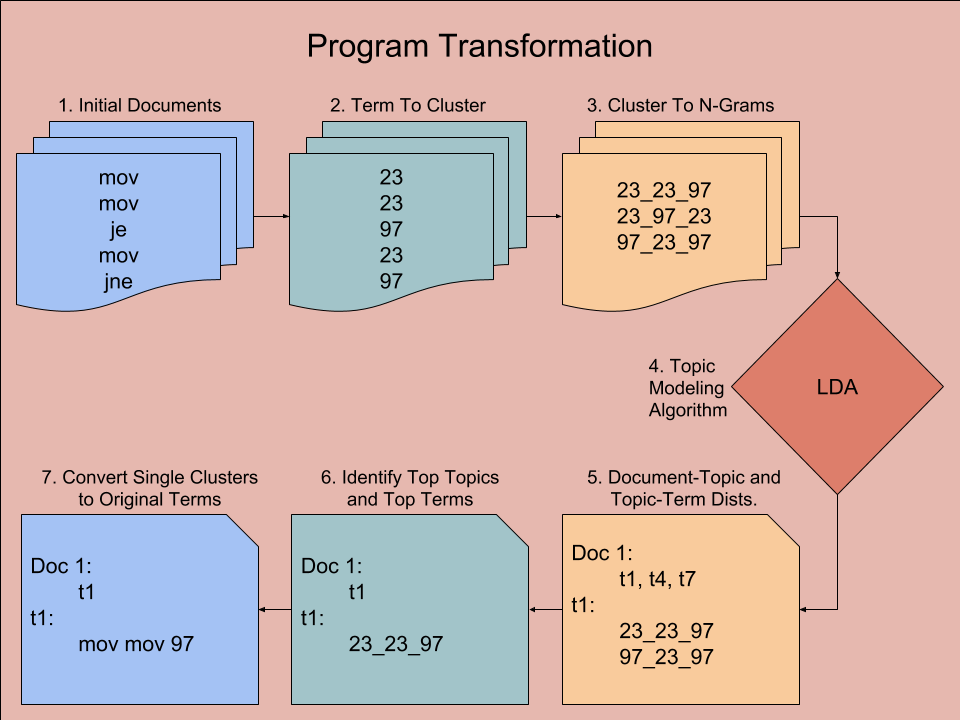
\includegraphics[width=\linewidth]{./figures/transform.png}
  \caption{Flowchart detailing the flow and transformation of information across the entire process. Documents are transformed and analyzed using LDA, and then the transformations are undone to allow for fine-grain interpretability.}
  \label{fig:flow}
\end{figure}

The system described fulfills the requirements of extracting interpretable behavioral components of software in an unsupervised manner. The details of each of the system's components is discussed below.

\subsection{Data and Assembly Instructions}
	\begin{figure}
  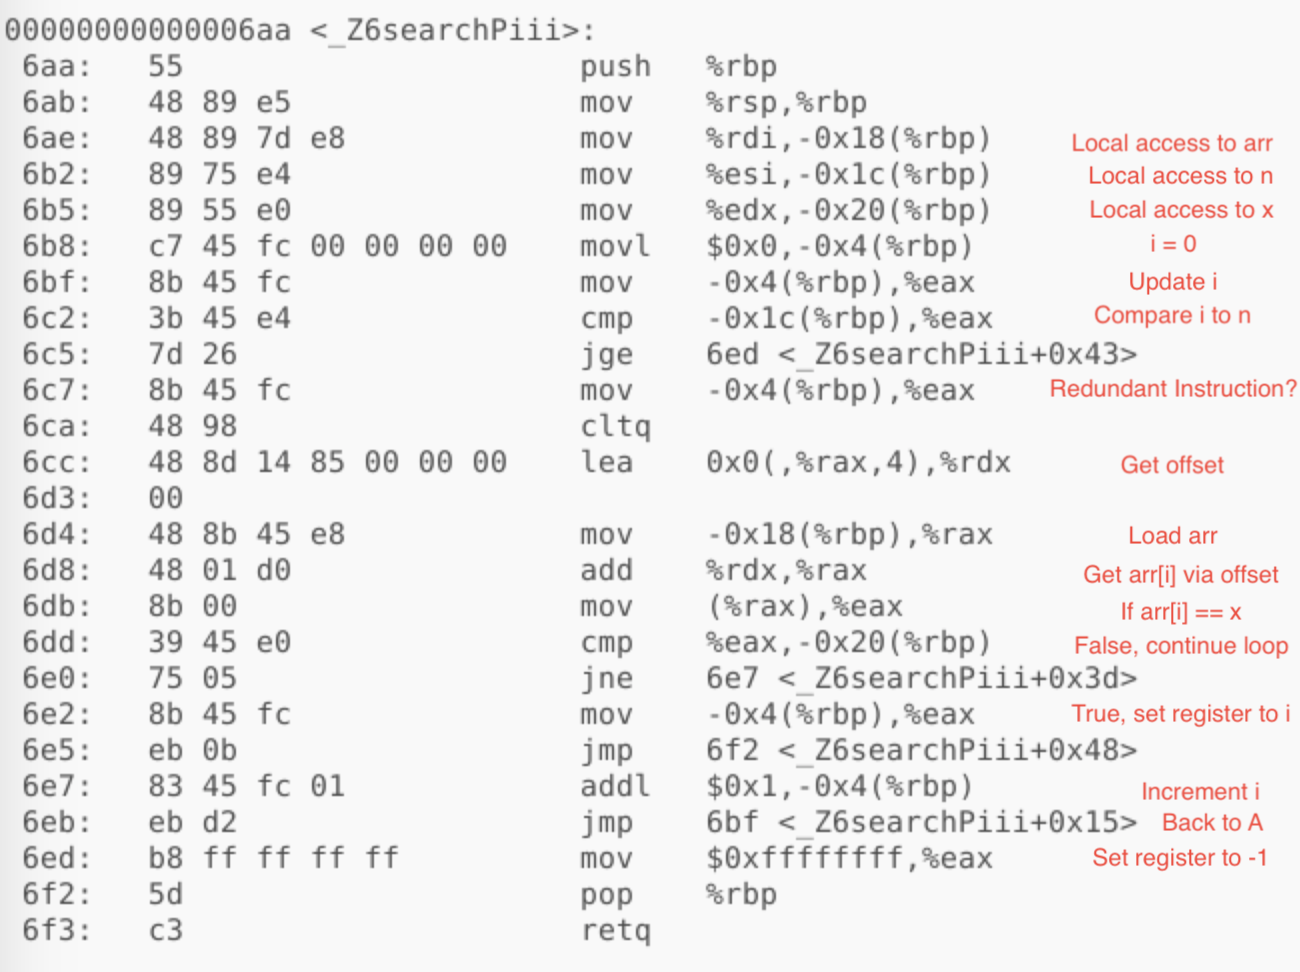
\includegraphics[width=\linewidth]{./figures/Annotated_search_assembly_ATT.png}
  \caption{Annotated version of Linear Search's search function in assembly. Similarities were found in sorting functions with the primary difference being sections of data modification and multiple for-loops.}
  \label{fig:search}
\end{figure}

Before moving towards a specific model, we first wished to see what differences occur between programs with different purposes, such as sorting programs versus searching programs. These two types of programs are two fundamental concepts of many programs and were identified as appropriate vehicles to develop and understand this approach. Initial analyses were performed on a small dataset collected from the Geeks4Geeks Website \cite{geeks}, where C++ samples of major sorting and searching algorithms were downloaded and compiled onto a Ubuntu 64-bit system. A larger dataset was later utilized using ByteWeight's dataset \cite{bao2014byteweight}. 

To understand the differences between programs, we first closely examined one sorting and one searching program to see what differences might exist between their assemblies. Figure \ref{fig:search} shows an annotated version of Linear Search's search function, and when compared with a sorting program such as Selection Sort (which effectively contains a modified version of a linear search as it sorts the program), the primary differences found were multiple for-loops and sections for data modification, something which most, if not all, sorting programs should have, but no realistic searching programs should have, as efficient searching programs should only have one loop, and should not be modifying the data. This formed the basis of our argument: \textit{Programs can be thought of as being made up of a set of underlying components, and these components are in some way shared across all programs.} The order and frequency in which these components occur can enable behavioral comparisons between programs, and understanding the components themselves allows for fine-grain understanding of behavior. The system presented in this work only incorporates the commands themselves so that basic functionality of the software could be understood. Incorporating arguments would allow for a better understanding of command targets (such as specific registers or functions), but would first require abstracting these in a way similar to Symbolic Execution so that program-to-program comparisons can be maintained.

	
\subsection{Word2Vec Embeddings and Clustering}
	Assembly commands also deserve their own form of abstraction, primarily in the context in which they are used. Using sorting as an example, changing a single greater-than comparator to a less-than comparator does not change the fact that the program is sorting, all it changes is the sorting order from increasing to decreasing. In order to allow for greater robustness in program types, our system must be able to take the context in which a specific command is used into account. One of the most effective methods of this is Word2Vec \cite{mikolov2013distributed}, which is able to identify terms used in similar contexts and can even be extrapolated to higher-level relationships (such as man->woman being similar to king->queen). Using the embeddings learned from Word2Vec, we gain a numerical representation of each command's context, with more similar commands sharing similar contexts. 

The small-scale experiment results of Word2Vec are shown in the T-SNE plot in Figure \ref{fig:tsne}. The findings shown in the plot correspond relatively well to human understanding, as most of the jump comparators are close to each other (jle, jg, jge); however, je is actually quite far from the rest of the comparators. We believe this is the result of the small data sample (16 documents) skewing the results. Once the high-dimensional embedding representations of terms were found, we applied hierarchical clustering to them and used our best understanding of command similarity to define the cutting point. Though this approach was adequate to confirm the validity of our system, a more formal study of assembly language usage would be preferred to validate the contexts in which commands are used and how they relate to one another. The results of this are shown in Figure \ref{fig:clust}. Both of these processes are repeated for the larger (about 850 documents) dataset, though the results of those embeddings and clusters are not shown in this paper as the images are too cluttered to be meaningfully presented.

\begin{figure}
  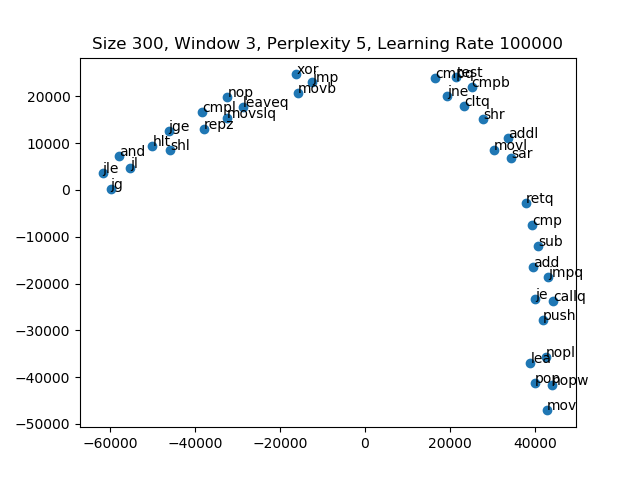
\includegraphics[width=\linewidth]{./figures/tsne_small.png}
  \caption{T-SNE plot of small-scale data Word2Vec results.}
  \label{fig:tsne}
\end{figure}

\begin{figure}
  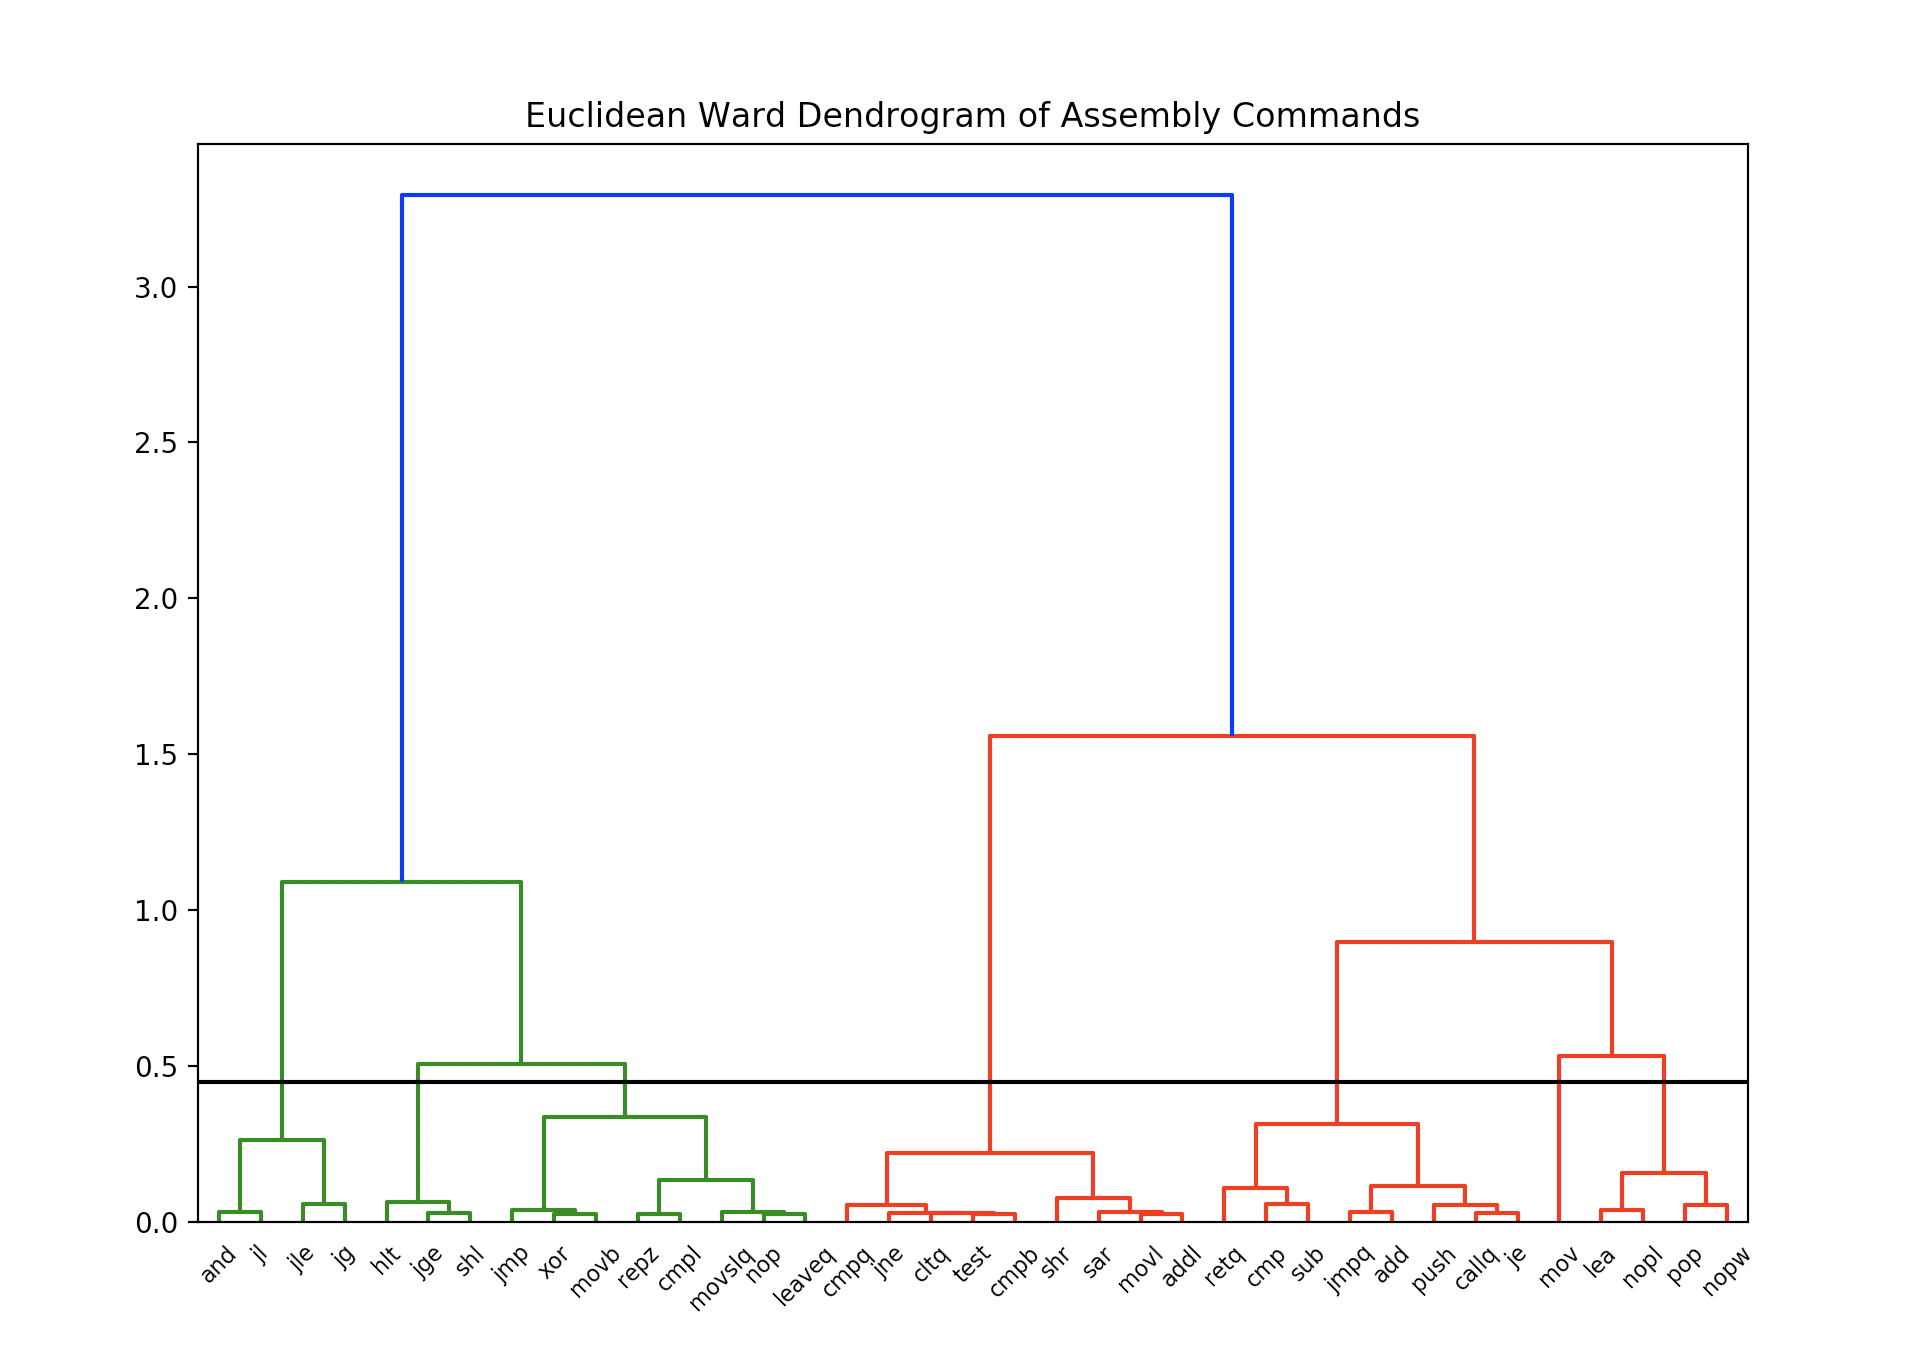
\includegraphics[width=\linewidth]{./figures/clust_small.png}
  \caption{Hierarchical Clustering results of the small dataset.}
  \label{fig:clust}
\end{figure}
	
\subsection{N-Grams}
	After converting the assembly commands to their corresponding cluster ID's, a way to have components with interpretable behavior was desired. Individual commands carry little meaning beyond their intended purpose, as one cannot extrapolate the meaning of a single "mov" or "pop" statement beyond its intended purpose; however, one can derive greater understanding of behavior through sequences of terms rather than singular terms. This brings us to N-Grams, which are sequences of terms (in this case cluster IDs) adjacent to each other (e.g. the 2-grams of "mov addl mov pop" are "mov addl", "addl mov", and "mov pop"). Smaller N-grams are less interpretable than large N-grams, and so a sizeable N must be chosen to maintain interpretability, which for our purposes means N = 8. Unfortunately, this has the side effect of drastically increasing vocabulary, so some caution must be taken.
	
\subsection{LDA and hLDA}
	As we defined programs as being made up sets of behavioral components, and those behaviors are largely unknown to us, we needed a system which would allow us to extract those behaviors in an unsupervised manner. This is actually a well-studied area in languages with NLP approaches in the area called Topic Modeling. Blei \textit{et al.} \cite{blei2003latent} developed a method for unsupervised topic modeling called Latent Dirichlet Allocation and would later expand upon it by developing Hierarchical Latent Dirichlet Allocation (hLDA) \cite{griffiths2004hierarchical}. LDA essentially considers each document to be made up of some weighting of latent topics and each topic to be made up of some weighting of terms. Then, it finds the distribution on these weightings which can be used for inference. hLDA is a hierarchical variant which adds the idea that topics are actually structured in a hierarchy. This approach is more akin to software than flat topics; however, there are not many performant hLDA libraries available for larger datasets. This led to a focus on LDA for the time being. LDA has more performant versions available, such as Microsoft's LightLDA \cite{yuan2015lightlda}, which we utilize in our analyses on the larger dataset.
	

	
\section{Results}\label{results}
	The following are the results of applying our approach to both small-scale and large-scale data, with small-scale referring to the 16 sorting and searching program samples from GeeksForGeeks (with an end-goal to differentiate sorting and searching programs), while the large-scale also includes the data files from ByteWeight, which consist of a variety of binutils programs compiled using different compilers and different compiler arguments.

\subsection{Small-Scale Results}

Below are the results of small-scale experiments with LDA and hLDA, both of which perform quite well.

\subsubsection{LDA Results}

\begin{figure}
  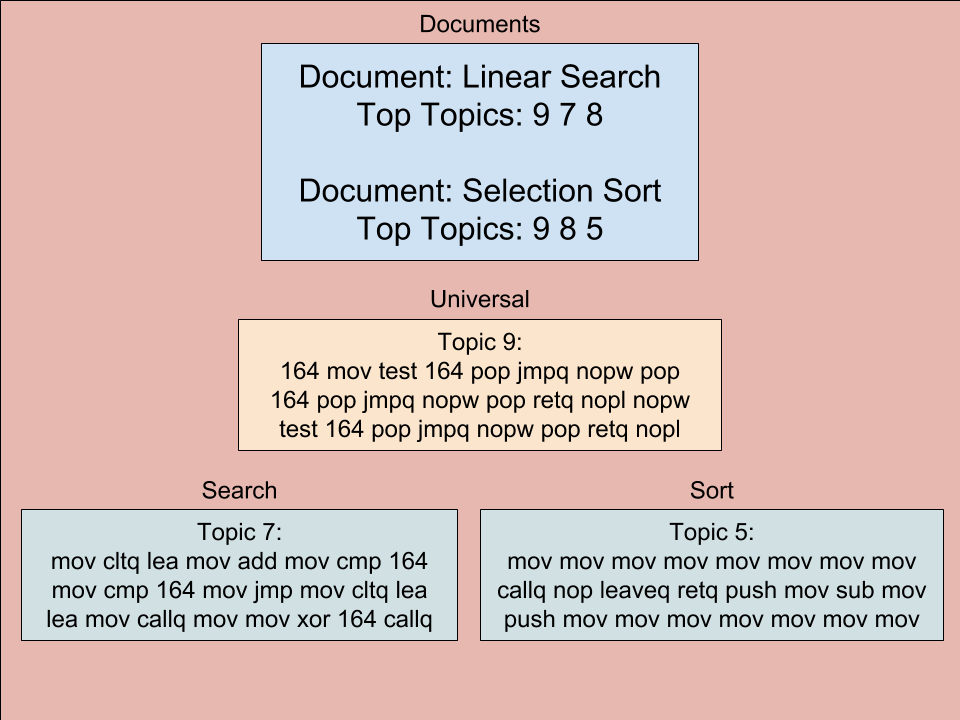
\includegraphics[width=\linewidth]{./figures/ss_fig.png}
  \caption{Side-by-side comparison of Linear Search and Selection Sort. Selection sort can be thought to contain the entirety of linear search (as a slightly modified linear search is used in the selection sort algorithm), so these two programs will be the most similar while still having different purposes.}
  \label{fig:small_lda}
\end{figure}

\begin{table}[]
\centering
\caption{Final results of small-scale LDA model. The top topics are determined based on the learned document-topic distribution. Focus on specific topics is contained in Figure \ref{fig:small_lda}. Hyperparameters for these results were the following: Number of topics = 13, $\alpha = 1e-10, \beta = 0.1$}
$\begin{array}{		l	l	l	l	}
\multicolumn{4}{c}{$LDA Table Results$}                  \\ \hline
$Program$                & \multicolumn{3}{c}{$Top Topics$} \\ \hline
Binary Search          & 9        & 7         & 12       \\ \hline
Interpolation Search   & 9        & 2         & 7        \\ \hline
Linear Search          & 9        & 7         & 8        \\ \hline
Rec. Linear Search     & 9        & 11        & 12       \\ \hline
Jump Search            & 9        & 11        & 19       \\ \hline
Exponential Search     & 9        & 7         & 12       \\ \hline
Bubble Sort            & 9        & 8         & 5        \\ \hline
Rec. Bubble Sort       & 9        & 8         & 5        \\ \hline
Merge Sort             & 6        & 9         & 0        \\ \hline
Rec. Merge Sort        & 6        & 9         & 0        \\ \hline
Quick Sort             & 5        & 9         & 11       \\ \hline
Rec. Quick Sort        & 9        & 5         & 8        \\ \hline
Insertion Sort         & 9        & 4         & 8        \\ \hline
Rec. Insertion Sort       & 9        & 4         & 11       \\ \hline
Selection Sort         & 9        & 8         & 5        \\ \hline
Rec. Heap Sort         & 9        & 1         & 11       \\ \hline
\end{array}$
\label{tab:small_lda_tab}
\end{table}

Figure \ref{fig:small_lda} shows a comparison between the Linear Search and Selection Sort programs with n-grams of size 8. The three topics displayed below were the most significant topics. Topic 9 was held as the most heavily weighted topic for most of the programs, and was the second most significant for three of the sixteen. Topics 7 and 5 were found to be the key differentiators between sorting and searching programs, with topic 7 being found in the majority of searching programs and no sorting programs, and topic 5 being found in many sorting programs and no searching programs. The full small-scale results are shown in Table \ref{tab:small_lda_tab}. Note the fact that topic 5 contains indications of heavy data modification (through the large number of mov statements), while topic 7 makes note of array comparisons in a loop.

\subsubsection{hLDA Results}

\begin{table}[]
\centering
\caption{Final results of small-scale hLDA model. Each document is a leaf node in a hierarchy of topics, so those at the same leaf node are most similar. Hyperparameters for these results were the following: Number of levels = 3, number of samples = 500, $\alpha = 10, \gamma = 1, \beta = 0.1$}
$\begin{array}{	l	c	}
\multicolumn{2}{c}{$hLDA Table Results$}                  \\ \hline
$Program$                & $Deepest Topic in Hierarchy$ \\ \hline
Binary Search          & 8       \\ \hline
Interpolation Search   & 8        \\ \hline
Linear Search          & 8        \\ \hline
Rec. Linear Search     & 8       \\ \hline
Jump Search            & 8       \\ \hline
Exponential Search     & 8       \\ \hline
Merge Sort             & 4       \\ \hline
Rec. Merge Sort        & 4        \\ \hline
Bubble Sort            & 10       \\ \hline
Rec. Bubble Sort       & 10        \\ \hline
Quick Sort             & 10       \\ \hline
Rec. Quick Sort        & 10        \\ \hline
Selection Sort         & 10        \\ \hline
Insertion Sort         & 6        \\ \hline
Rec. Insertion Sort       & 6      \\ \hline
Rec. Heap Sort         & 6       \\ \hline
\end{array}$
\label{tab:small_hlda_tab}
\end{table}

Table \ref{tab:small_hlda_tab} shows the final topics corresponding to each of the programs from hLDA. One can observe that all search programs were successfully isolated from all sort programs. In addition, various recursive versions of programs were matched with their non-recursive versions. These results are very promising and clearly indicate tremendous potential for this approach.

\subsection{Large-Scale Results}

This section discusses the results of the large-scale LDA experiments.

\begin{figure}
  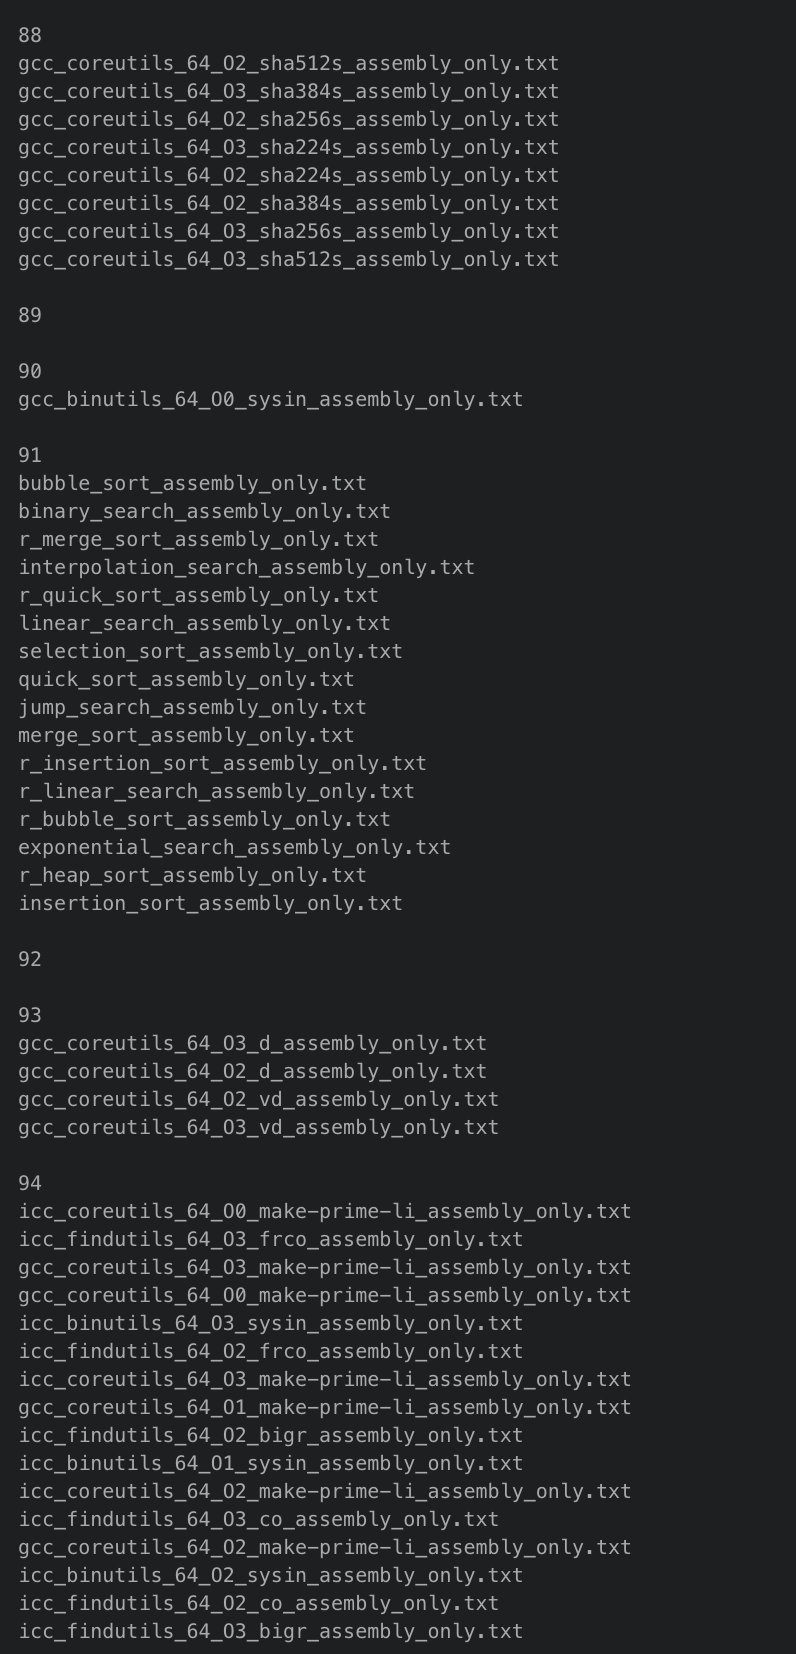
\includegraphics[width=\linewidth]{./figures/large_lda_top_level.png}
  \caption{Documents placed into bins corresponding to their highest-weighted topic. All sorting and searching programs are placed into the same bin, with no other programs being placed within it.}
  \label{fig:large_lda}
\end{figure}

\begin{table}[]
\centering
\caption{Final results of large-scale LDA model. The top topics are determined based on the learned document-topic distribution.  Hyperparameters for these results were the following: Number of topics = 100, $\alpha = 0.001, \beta = 0.001$. The - symbol means that no additional topics were formed as part of its weighting (due to their weights being too small).}
$\begin{array}{	l	l	l	l	l	l	}
\multicolumn{6}{c}{$LDA Table Results$}                  \\ \hline
$Program $               & \multicolumn{5}{c}{$Top Topics$} \\ \hline
Binary  Search          & 91        & 86         & 62 & 78 & 42       \\ \hline
Interpolation  Search   & 91        & 88         & 86 & 61 & 90        \\ \hline
Linear  Search          & 91        & 86         & 33 & 78 &  -      \\ \hline
Rec.  Linear  Search     & 91        & 61        & 86 & 89 & 20       \\ \hline
Jump  Search            & 91        & 78        & 86 & 89 & 27       \\ \hline
Exponential  Search     & 91        & 61         & 86 & 78 & 3       \\ \hline
Bubble  Sort            & 91        & 86         & 51 & 3 & -        \\ \hline
Rec.  Bubble  Sort       & 91        & 86         & 51 & 90 & 80        \\ \hline
Merge  Sort             & 91        & 86         & 61 & 74 & 20        \\ \hline
Rec.  Merge  Sort        & 91        & 86         & 61 & 74 & 20        \\ \hline
Quick  Sort             & 91        & 61         & 86 & 62 & -     \\ \hline
Rec.  Quick  Sort        & 91        & 61         & 86 & 62 & 24        \\ \hline
Insertion  Sort         & 91        & 86         & - & - & -        \\ \hline
Rec.  Insertion  Sort       & 91        & 86         & 61 & - & -       \\ \hline
Selection  Sort         & 91        & 86         & 61 & 80 & 90        \\ \hline
Rec.  Heap  Sort         & 91        & 86         & 61 & 20 & 56       \\ \hline
\end{array}$
\label{tab:large_lda_tab}
\end{table}

Figure \ref{fig:large_lda} shows a small subset of the large-scale results, namely the documents being sorted into bins based on what each document's highest-weighted topic was. As can be seen, all sorting and searching programs are placed in the same bin, with no other programs being placed with them. Additionally, examination of nearby bins reveals other successes, such as isolation of multiple types of hash functions, or different compiled versions of the same program (make-prime-li).

Table \ref{tab:large_lda_tab} details the results of the large-scale test for the original sorting and searching programs. The main difference of this test is to see what topics would be found when there are a wider variety of programs, and how the programs would relate to one another when scaling up. Results show programs pairing with their recursive versions somewhat less frequently, and there do not exist any major differentiators between the sorting and searching programs. That being said, all of the small-scale programs (sorting and searching programs of similar style and the same origin, compiler, and compiler arguments) were found to have the same most significant topic (topic 91). While not as strong as the small-scale results, they are still quite promising.
	
\section{Discussion}\label{discussion}
	The details of our experimental findings are discussed in this section, including the trade-offs between LDA and hLDA, and the differences between the small-scale and large-scale results.

\subsection{LDA and hLDA}
Results from the small-scale LDA and hLDA experiments were both incredibly promising, as both were able to identify topics which separated programs of different behaviors, fulfilling the goal of being able to learn interpretable behavior components from the assemblies of various programs. These components represent the key differences in behavior that would identify programs as being a sorting or searching program (or neither). Not only that, but this system enables one to understand to what degree a program is of a certain type or what subtype it may belong to based on other programs of the same type, such as identifying a program as closer to binary search or linear search; however, it should be noted that these approaches do not come without their issues. Identifying the number of topics in LDA requires either hand-tuning or the use of a hyperparameter searching algorithm such as grid search to optimize perplexity. Alpha and beta also require tuning, but the number of topics has the strongest effect on model results. Finding the hyperparameters for hLDA would require something similar except more parameters need to be found. These problems are not unique to LDA and hLDA however, as almost all machine learning algorithms require some form of hyperparameter tuning \cite{hype}. Most systems utilizing machine learning to identify these components would require some form of hyperparameter search.

Determining the number of topics is a difficult problem for LDA as it may change depending on the number of documents and their contents. One could perform a hyperparameter grid search, using perplexity as the basis for determining the optimal number of topics; however, perplexity may not be an adequate measure. Change \textit{et al.} \cite{chang2009reading} found that perplexity did not correlate with human judgment in the topics found very well. While there may be other methods for determining the adequacy of a number of topics, it may be more beneficial to use the Hierarchical Dirichlet Process \cite{teh2005sharing}, as it generates similar results compared to LDA, but the number of topics is no longer a hyperparameter and is instead determined by the model. Applying HDP instead of LDA may be more beneficial for determining the number of topics; however, there are still other hyperparameters which need to be tuned, and HDP may not be as performant as LDA.

It is clear that hLDA (Table \ref{tab:small_hlda_tab}) performs better as a classifier for sorting and searching programs compared to LDA (Table \ref{tab:small_lda_tab}), as it is able to create a complete and clear separation between sorting and searching programs with additional insights for recursive non-recursive pairs. In addition, hLDA's innate hierarchical structuring of components is more appropriate to our idea of behavioral components having a hierarchical relationship; that being said, LDA's result structure is more directly interpretable in terms of the components that make up a given program. It also gives a clearer picture in terms of understanding which components make up a given document and to what weighting they have. In addition, hLDA is much less scalable than LDA, as it requires iterating through the length of every document multiple times. We found that it runs approximately 10-15x longer than LDA with the trade-off of achieving better results, though the results for a given hyperparameter set were more inconsistent with hLDA than LDA, which is most likely the result of hLDA making use of additional random variables in its model, decreasing its consistency in results. With these ideas in mind, we decided to maintain LDA for the large-scale experiment until such a time as a more performant hLDA library is made available or better hardware is found, leaving this as an area to study in the future.

\subsection{Large-Scale LDA}
As performance was poor using Python for LDA from GuidedLDA \cite{guidedlda}, we searched for more efficient libraries for LDA and found Microsoft's LightLDA program, written in C++ to be multi-threaded and able to be distributed to multiple machines. We thought this to be the most appropriate package to use moving forward into any larger data sets.

At a high-level, the large-scale results were quite good, as all of the sorting and searching programs were found to have the same highest-weighted topic. As indicated in Figure \ref{fig:large_lda}, no other programs were binned with them. In addition, other similar programs were found to be mapped together, such as different versions of hashing functions (sha512s, sha256s, etc.) or the same program with different arguments or compilers (make-prime-li). This can give potentially immediate insights into a program's point of origin in relation to other programs and its behavior. This also confirms the system is stable under different compilers and compiler options, which would prove very beneficial for maintaining robustness in applications related to malware analysis.

At a finer granularity, the system does not perform as well on the small-scale experiment. Most of the searching and sorting programs have a high level of interconnectivity in terms of shared top topics, and some of the recursive versions are matched with their non-recursive forms (such as quick sort and merge sort), but there does not exist any single identifiable topic for sorting or searching which might be a key differentiator between them. This is most likely due to the heavy weighting of program types, as the majority of programs are from the ByteWeight data set, and many of the programs are duplicates with different compilers or compiler arguments, thereby shifting many of the topics found to be more closely related to them than a small subset of sorting and searching programs. Increasing the number of topics could potentially improve this, but there is a bound to the effectiveness of increasing the number of flat topics, and as we discuss later, using a hyperparameter search to optimize perplexity may not lead to the correct topics.

Despite there being no key differentiators at the large-scale, this system still provides the basis by which one could, in an unsupervised manner, find interpretable behavioral components of programs and compare programs based on these shared or unshared components. Being able to extract these components in an unsupervised way is the key to creating new insights, as much of the underlying behavioral differences between programs remain unknown to us in an understandable way, despite much previous work being done in studying their behavioral differences in attempts to classify them. This system also provides a strong foundation on which many subsystems can be added to improve performance or gain greater insight into program behavior.
	
\section{Future Work}\label{future_work}
	There are a multitude of directions towards which this work could be extended, with several of them being discussed below, along with any potential roadblocks they may have.

%\subsection{Number of Topics and the Hierarchical Dirichlet Process}
%	Determining the number of topics is a difficult problem for LDA as it may change depending on the number of documents and their contents. One could perform a hyperparameter grid search, using perplexity as the basis for determining the optimal number of topics; however, perplexity may not be an adequate measure. Change \textit{et al.} \cite{chang2009reading} found that perplexity didn't correlate with human judgment in the topics found very well. While there may be other methods for determining the adequacy of a number of topics, it may be more beneficial to use the Hierarchical Dirichlet Process \cite{teh2005sharing}, as it generates similar results compared to LDA, but the number of topics is no longer a hyperparameter and is instead determined by the model. Applying HDP instead of LDA may be more beneficial for determining the number of topics; however, there are still other hyperparameters which need to be tuned, and HDP may not be as performant as LDA.
	
%\subsection{Abstract Components}
%	The results of LDA are a per-document distribution on the topics, as well as a per-topic distribution on the terms. Hypothetically, one could discretize these distributions and apply LDA again, creating another latent topic set by which one could describe the previous topics. The application of this to language is clear, as the initial topics are then mixed to create more abstract versions. For the purposes of understanding programs, this could be thought of as combining behavioral components into more abstract, yet still interpretable, higher-level components. This would be a interesting direction to focus in, as it could be used to describe higher-order functions that human experts unfamiliar to assembly instructions could still understand.
	
%\subsection{Contextual Analysis}
	In its current state, our system largely focuses on behavior as separate from context, but combining this with a contextual analysis system would greatly enhance understanding of behavior. For one, incorporating the arguments of the instructions would give greater clarity in terms of the actual operations and machine state being altered by the program itself. Beyond the instructions themselves, incorporating the environment and machine state into the model (such as the physical environment around the machine, the type of machine, or the machine's operating system) would assist in generating a system-wide view of behavior and how its state is modified by the underlying behavioral components. This would improve understanding of software and its behavior and would be particularly beneficial for isolating malware and determining its severity in a given context.
	
%\subsection{Application to Dynamic Analysis}
	Our current approach focuses on statically derived assembly commands taken from the objdumps of binary executables; however, this does not give a complete picture of the software and has multiple shortcomings, such as ignoring function boundaries and ignoring jump locations. If a dynamic trace were collected through execution of the programs such that each program was represented by the assembly commands used in the order of their execution throughout the entire runtime, one would thereby gain insights into the function boundaries and jump statements. Unfortunately, collecting these dynamic traces takes time, as each program must be run multiple times with different arguments, as not all commands are run in every execution. As concluded in \cite{santos2013opem}, a combined static-dynamic approach would most likely be best.
	
%\subsection{Large-Scale hLDA}
%	As it currently stands, there are a multitude of libraries built for large-scale LDA, such as Microsoft's LightLDA; however, the results we gained from using hLDA seemed more closely aligned with what we'd prefer as a way to understand programs in relation to one another while still understanding their underlying behavioral components. It would be interesting to repeat the analysis for the large-scale data set using hLDA if a more efficient and scalable version could be created, as hierarchical components are a more appropriate conceptualization of program behavior than flat components, as programs are typically created in a hierarchical and object-oriented framework.
	
%\subsection{Malware Analysis}
	This paper details an initial proof of concept on a small-scale sort versus search data set, with additional testing on a large-scale data set. While this study did not focus on malware, its applicability to the malware analysis domain is clear. The difficulty with studying malware stems from safely acquiring copies of malware and using them for study. The most widely available data set is Microsoft's Kaggle data set \cite{kaggle}, which can be used to try to classify malware into one of nine families. This would be the most immediately useful data set to study, though due to its size, performance may become an issue if one does not use an efficient library. The issue with this data set is its lack of benign program samples, which would be necessary if trying to find differentiators between malware and non-malware programs and their corresponding behaviors. One could add the ByteWeight data set to it, but more varied programs and more examples of commercial software would assist in making the approach generalizable.
	
\section{Conclusion}\label{conclusion}
	Understanding a software's behavior, both intrinsically and in relation to other software, is an important stepping stone towards effective program behavioral analysis and can give greater insights into understanding how programs relate to one another. We detail the importance of this understanding and of having interpretable behavioral components and presented our system LIBCAISE, a novel approach to identifying behavioral components in software by applying NLP techniques to the domain of software analysis. While there are various tradeoffs to our approach, it succinctly captures multi-level interpretable software behavior and lays important groundwork on which a variety of directions may extend from.
	
	




% An example of a floating figure using the graphicx package.
% Note that \label must occur AFTER (or within) \caption.
% For figures, \caption should occur after the \includegraphics.
% Note that IEEEtran v1.7 and later has special internal code that
% is designed to preserve the operation of \label within \caption
% even when the captionsoff option is in effect. However, because
% of issues like this, it may be the safest practice to put all your
% \label just after \caption rather than within \caption{}.
%
% Reminder: the "draftcls" or "draftclsnofoot", not "draft", class
% option should be used if it is desired that the figures are to be
% displayed while in draft mode.
%
%\begin{figure}[!t]
%\centering
%\includegraphics[width=2.5in]{myfigure}
% where an .eps filename suffix will be assumed under latex, 
% and a .pdf suffix will be assumed for pdflatex; or what has been declared
% via \DeclareGraphicsExtensions.
%\caption{Simulation results for the network.}
%\label{fig_sim}
%\end{figure}

% Note that the IEEE typically puts floats only at the top, even when this
% results in a large percentage of a column being occupied by floats.
% However, the Computer Society has been known to put floats at the bottom.


% An example of a double column floating figure using two subfigures.
% (The subfig.sty package must be loaded for this to work.)
% The subfigure \label commands are set within each subfloat command,
% and the \label for the overall figure must come after \caption.
% \hfil is used as a separator to get equal spacing.
% Watch out that the combined width of all the subfigures on a 
% line do not exceed the text width or a line break will occur.
%
%\begin{figure*}[!t]
%\centering
%\subfloat[Case I]{\includegraphics[width=2.5in]{box}%
%\label{fig_first_case}}
%\hfil
%\subfloat[Case II]{\includegraphics[width=2.5in]{box}%
%\label{fig_second_case}}
%\caption{Simulation results for the network.}
%\label{fig_sim}
%\end{figure*}
%
% Note that often IEEE papers with subfigures do not employ subfigure
% captions (using the optional argument to \subfloat[]), but instead will
% reference/describe all of them (a), (b), etc., within the main caption.
% Be aware that for subfig.sty to generate the (a), (b), etc., subfigure
% labels, the optional argument to \subfloat must be present. If a
% subcaption is not desired, just leave its contents blank,
% e.g., \subfloat[].


% An example of a floating table. Note that, for IEEE style tables, the
% \caption command should come BEFORE the table and, given that table
% captions serve much like titles, are usually capitalized except for words
% such as a, an, and, as, at, but, by, for, in, nor, of, on, or, the, to
% and up, which are usually not capitalized unless they are the first or
% last word of the caption. Table text will default to \footnotesize as
% the IEEE normally uses this smaller font for tables.
% The \label must come after \caption as always.
%
%\begin{table}[!t]
%% increase table row spacing, adjust to taste
%\renewcommand{\arraystretch}{1.3}
% if using array.sty, it might be a good idea to tweak the value of
% \extrarowheight as needed to properly center the text within the cells
%\caption{An Example of a Table}
%\label{table_example}
%\centering
%% Some packages, such as MDW tools, offer better commands for making tables
%% than the plain LaTeX2e tabular which is used here.
%\begin{tabular}{|c||c|}
%\hline
%One & Two\\
%\hline
%Three & Four\\
%\hline
%\end{tabular}
%\end{table}


% Note that the IEEE does not put floats in the very first column
% - or typically anywhere on the first page for that matter. Also,
% in-text middle ("here") positioning is typically not used, but it
% is allowed and encouraged for Computer Society conferences (but
% not Computer Society journals). Most IEEE journals/conferences use
% top floats exclusively. 
% Note that, LaTeX2e, unlike IEEE journals/conferences, places
% footnotes above bottom floats. This can be corrected via the
% \fnbelowfloat command of the stfloats package.





% if have a single appendix:
%\appendix[Proof of the Zonklar Equations]
% or
%\appendix  % for no appendix heading
% do not use \section anymore after \appendix, only \section*
% is possibly needed

% use appendices with more than one appendix
% then use \section to start each appendix
% you must declare a \section before using any
% \subsection or using \label (\appendices by itself
% starts a section numbered zero.)
%


\appendices
%\section{Proof of the First Zonklar Equation}
%Appendix one text goes here.
%
% you can choose not to have a title for an appendix
% if you want by leaving the argument blank
%\section{}
%Appendix two text goes here.



% use section* for acknowledgment
\ifCLASSOPTIONcompsoc
  % The Computer Society usually uses the plural form
  \section*{Acknowledgments}
\else
  % regular IEEE prefers the singular form
  \section*{Acknowledgment}
\fi


The authors would like to thank the University of Cincinnati (UC), Air Force Research Laboratory (AFRL), and Defense Associated Graduate Student Innovators (DAGSI) for providing the resources necessary to complete this work and for the collaboration with members of AFRL. This work was funded in part by DAGSI award number RY12-UC-18-4. Code and data available on GitHub \footnote{https://github.com/jgreer013/libcaise}


% Can use something like this to put references on a page
% by themselves when using endfloat and the captionsoff option.
\ifCLASSOPTIONcaptionsoff
  \newpage
\fi

\bibliographystyle{./bib/IEEEtran.bst}
\bibliography{./bib/biblio.bib}


% biography section
% 
% If you have an EPS/PDF photo (graphicx package needed) extra braces are
% needed around the contents of the optional argument to biography to prevent
% the LaTeX parser from getting confused when it sees the complicated
% \includegraphics command within an optional argument. (You could create
% your own custom macro containing the \includegraphics command to make things
% simpler here.)
%\begin{IEEEbiography}[{\includegraphics[width=1in,height=1.25in,clip,keepaspectratio]{mshell}}]{Michael Shell}
% or if you just want to reserve a space for a photo:

\newpage

\begin{IEEEbiographynophoto}{Jeremiah Greer}
received in B.S. degree in Computer Science from the University of Cincinnati, Cincinnati, Ohio, in 2018, and is currently pursuing his M.S. degree in Computer Science at the University of Cincinnati. He has accepted a position at Microsoft in Redmond for Fall 2019. His current research interests include natural language processing, neural networks, software and malware analysis, and artificial intelligence, particularly in game AI.
\end{IEEEbiographynophoto}
\vskip 0pt plus -1fil
% if you will not have a photo at all:
\begin{IEEEbiographynophoto}{Rashmi Jha}
is an Associate Professor in Electrical Engineering and Computer Science Department at the University of Cincinnati. She worked as a Process Integration Engineer for Advanced CMOS technologies at IBM Microelectronics, between 2006-2008. She finished her Ph.D. and M.S. in Electrical Engineering from North Carolina State University in 2006 and 2003, respectively, and B.Tech. in Electrical Engineering from IIT Kharagpur, India in 2000. She has been granted 12 US patents and has authored/co-authored several publications. She has been a recipient of Summer Faculty Fellowship award from AFOSR in 2017, CAREER Award from the National Science Foundation (NSF) in 2013, IBM Faculty Award in 2012, IBM Invention Achievement Award in 2007. She is the director of Microelectronics and Integrated-systems with Neuro-centric Devices (MIND) laboratory at the University of Cincinnati. Her current research interests lie in the areas of Artificial Intelligence, Cybersecurity, Neuromorphic SoC, Emerging Logic and Memory Devices, Hardware Security, and Neuroelectronics.
\end{IEEEbiographynophoto}
\vskip 0pt plus -1fil
% insert where needed to balance the two columns on the last page with
% biographies
%\newpage

\begin{IEEEbiographynophoto}{Anca Ralescu}
is a Full Professor in the EECS Department, University of Cincinnati, which she joined in 1983.  She holds degrees in Mathematics from University of Bucharest, Romania (BS, 1972), and Indiana University, Bloomington (MA, 1980, PhD 1983).  She currently heads the Machine Learning and Computational Intelligence Laboratory in the EECS Department, where with her students she is involved in machine learning research with applications to image understanding, text understanding, and cyber-security. Other research interests include brain-computer interface, and artificial intelligence. During 1991-1995 Dr. Ralescu was the Assistant Director of the Laboratory for International Fuzzy Engineering, Yokohama, Japan.  She held visiting positions at various universities, including University of Bristol, UK, Tokyo Institute of Technology, University of Oviedo, Spain, Osaka University, and ParisTech ENST, France.
\end{IEEEbiographynophoto}
\vskip 0pt plus -1fil
\begin{IEEEbiographynophoto}{Temesguen Messay-Kebede}
is a former faculty in the Electrical and Computer Engineering at the University of Dayton. He is currently a Research Engineer for the Avionics Cyber Protection Team in the Avionics Vulnerability Mitigation Branch, Sensors Directorate, at Wright-Patterson Air Force Base in Dayton, Ohio. He studied Electrical and Computer Engineering at the University of Dayton and he obtained his Ph.D. in December 2014. His research areas include pattern recognition, machine learning, image processing and understanding, robotics and cyber-security.
\end{IEEEbiographynophoto}
\vskip 0pt plus -1fil
\begin{IEEEbiographynophoto}{David Kapp}
is the Avionics Cyber Protection Team Lead in the Avionics Vulnerability Mitigation Branch, Sensors Directorate, at Wright-Patterson Air Force Base in Dayton, Ohio. Dr. Kapp has spent the last eighteen (18) years performing research and development in novel software protection and anti-tamper solutions for the DoD. His passion is building biologically-inspired adaptable and resilient cyber protection systems. He holds a Ph.D. in Electrical Engineering from Virginia Tech, where he specialized in electromagnetic scattering from randomly rough surfaces.
\end{IEEEbiographynophoto}

% You can push biographies down or up by placing
% a \vfill before or after them. The appropriate
% use of \vfill depends on what kind of text is
% on the last page and whether or not the columns
% are being equalized.

%\vfill

% Can be used to pull up biographies so that the bottom of the last one
% is flush with the other column.
%\enlargethispage{-5in}


% that's all folks
\end{document}


